% --------------------------------------------------------------
% This is all preamble stuff that you don't have to worry about.
% Head down to where it says "Start here"
% --------------------------------------------------------------
 
\documentclass[12pt]{article}
 
\usepackage[margin=1in]{geometry} 
\usepackage{amsmath,amsthm,amssymb}
\usepackage{graphicx}
\usepackage{enumitem}
\usepackage{enumerate}
\usepackage{pifont}
\usepackage{xcolor}
\usepackage{tikz}
\definecolor{smithblue}{HTML}{002855}
\definecolor{smithyellow}{HTML}{F2A900}

\def\firstcircle{(90:1.75cm) circle (2.5cm)}
\def\secondcircle{(210:1.75cm) circle (2.5cm)}
\def\thirdcircle{(330:1.75cm) circle (2.5cm)}

\usepackage[parfill]{parskip}
\parskip=\baselineskip
 
\newcommand{\N}{\mathbb{N}}
\newcommand{\Z}{\mathbb{Z}}
 
\newenvironment{exercise}[2][Exercise]{\begin{trivlist}
\item[\hskip \labelsep {\bfseries #1}\hskip \labelsep {\bfseries #2.}]}{\end{trivlist}}

\newenvironment{solution}[1][{\color{red} Solution:}]{\begin{trivlist}
\item[\hskip \labelsep {\bfseries #1}\hskip \labelsep {\bfseries}]}{\end{trivlist}}

\usepackage{fancyhdr}
\pagestyle{fancy}
\lhead{Submitted by: \ Sabrina Hatch\\
\collaborators}
\rhead{CSC250 Spring 2023 - Assignment 3\\
\today{}}
\cfoot{p. \thepage}
\renewcommand{\headrulewidth}{0.4pt}
\renewcommand{\footrulewidth}{0.4pt}

\begin{document}
 
% --------------------------------------------------------------
%                         Start here
% --------------------------------------------------------------


\newcommand{\studentName}{Sabrina Hatch} %replace with your name

\newcommand{\collaborators}{
	% Comment out the line below if you worked alone
	with \textit{Ramsha Rauf, Shalmon Mhanda}
	% Uncomment the line below if you worked alone
	% \textit{I did not collaborate with anyone on this assignment.}
}


% --------------
% Exercise 1
% --------------
\begin{exercise}{1}
Draw FAs that recognize each of the following languages using the specified number of states.
In all cases, the alphabet is $\Sigma = \{0, 1\}$.
\begin{enumerate}[(a)]
	\item $\{ w \in \Sigma^* \ | \ w \ ends \ with \ 11 \}$ using three states.
	% -------------------------------------------
	%  Write your answer to Q1a below
	% -------------------------------------------
	\begin{solution}
 \begin{center}
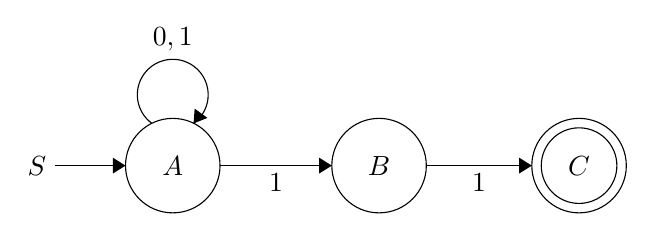
\begin{tikzpicture}[scale=0.2]
\tikzstyle{every node}+=[inner sep=0pt]
\draw [black] (10.8,-28.8) circle (3);
\draw (10.8,-28.8) node {$A$};
\draw [black] (23.9,-28.8) circle (3);
\draw (23.9,-28.8) node {$B$};
\draw [black] (36.6,-28.8) circle (3);
\draw (36.6,-28.8) node {$C$};
\draw [black] (36.6,-28.8) circle (2.4);
\draw [black] (13.8,-28.8) -- (20.9,-28.8);
\fill [black] (20.9,-28.8) -- (20.1,-28.3) -- (20.1,-29.3);
\draw (17.35,-29.3) node [below] {$1$};
\draw [black] (3.3,-28.8) -- (7.8,-28.8);
\draw (2.8,-28.8) node [left] {$S$};
\fill [black] (7.8,-28.8) -- (7,-28.3) -- (7,-29.3);
\draw [black] (9.477,-26.12) arc (234:-54:2.25);
\draw (10.8,-21.55) node [above] {$0,1$};
\fill [black] (12.12,-26.12) -- (13,-25.77) -- (12.19,-25.18);
\draw [black] (26.9,-28.8) -- (33.6,-28.8);
\fill [black] (33.6,-28.8) -- (32.8,-28.3) -- (32.8,-29.3);
\draw (30.25,-29.3) node [below] {$1$};
\end{tikzpicture}
\end{center}
	\end{solution}
	
	\item $\{ w \in \Sigma^* \ | \ w \ contains \ the \ substring \ 1010  \}$ using five states.
	% -------------------------------------------
	%  Write your answer to Q1b below
	% -------------------------------------------
	\begin{solution}
\begin{center}
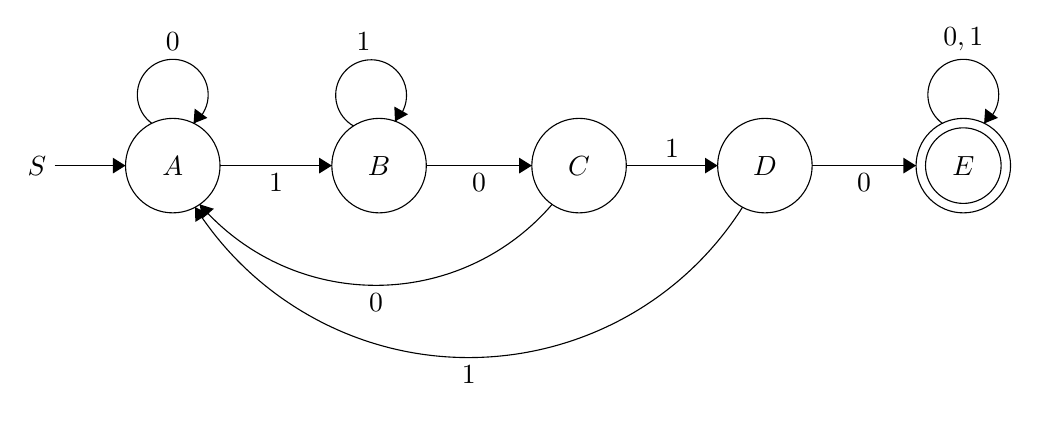
\begin{tikzpicture}[scale=0.2]
\tikzstyle{every node}+=[inner sep=0pt]
\draw [black] (10.8,-28.8) circle (3);
\draw (10.8,-28.8) node {$A$};
\draw [black] (23.9,-28.8) circle (3);
\draw (23.9,-28.8) node {$B$};
\draw [black] (36.6,-28.8) circle (3);
\draw (36.6,-28.8) node {$C$};
\draw [black] (48.4,-28.8) circle (3);
\draw (48.4,-28.8) node {$D$};
\draw [black] (61,-28.8) circle (3);
\draw (61,-28.8) node {$E$};
\draw [black] (61,-28.8) circle (2.4);
\draw [black] (13.8,-28.8) -- (20.9,-28.8);
\fill [black] (20.9,-28.8) -- (20.1,-28.3) -- (20.1,-29.3);
\draw (17.35,-29.3) node [below] {$1$};
\draw [black] (3.3,-28.8) -- (7.8,-28.8);
\draw (2.8,-28.8) node [left] {$S$};
\fill [black] (7.8,-28.8) -- (7,-28.3) -- (7,-29.3);
\draw [black] (9.477,-26.12) arc (234:-54:2.25);
\draw (10.8,-21.55) node [above] {$0$};
\fill [black] (12.12,-26.12) -- (13,-25.77) -- (12.19,-25.18);
\draw [black] (26.9,-28.8) -- (33.6,-28.8);
\fill [black] (33.6,-28.8) -- (32.8,-28.3) -- (32.8,-29.3);
\draw (30.25,-29.3) node [below] {$0$};
\draw [black] (22.285,-26.286) arc (240.44171:-47.55829:2.25);
\draw (22.91,-21.51) node [above] {$1$};
\fill [black] (24.91,-25.99) -- (25.74,-25.54) -- (24.87,-25.05);
\draw [black] (39.6,-28.8) -- (45.4,-28.8);
\fill [black] (45.4,-28.8) -- (44.6,-28.3) -- (44.6,-29.3);
\draw (42.5,-28.3) node [above] {$1$};
\draw [black] (51.4,-28.8) -- (58,-28.8);
\fill [black] (58,-28.8) -- (57.2,-28.3) -- (57.2,-29.3);
\draw (54.7,-29.3) node [below] {$0$};
\draw [black] (59.677,-26.12) arc (234:-54:2.25);
\draw (61,-21.55) node [above] {$0,1$};
\fill [black] (62.32,-26.12) -- (63.2,-25.77) -- (62.39,-25.18);
\draw [black] (34.89,-31.259) arc (-40.6383:-139.3617:14.747);
\fill [black] (12.51,-31.26) -- (12.65,-32.19) -- (13.41,-31.54);
\draw (23.7,-36.9) node [below] {$0$};
\draw [black] (46.981,-31.44) arc (-32.43899:-147.56101:20.594);
\fill [black] (12.22,-31.44) -- (12.23,-32.38) -- (13.07,-31.85);
\draw (29.6,-41.49) node [below] {$1$};
\end{tikzpicture}
\end{center}

	\end{solution}
	
	\item$\{ w \in \Sigma^* \ | \ w \ contains \ exactly \ two \ 0s, \ or \ at \ least \ two \ 1s \}$ using six states.
	% -------------------------------------------
	%  Write your answer to Q1c below
	% -------------------------------------------
	\begin{solution}
 
\begin{center}
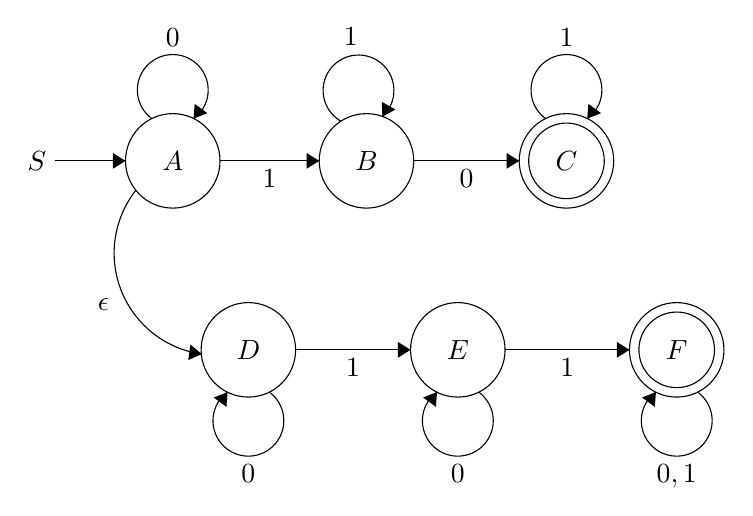
\begin{tikzpicture}[scale=0.2]
\tikzstyle{every node}+=[inner sep=0pt]
\draw [black] (11.9,-19.8) circle (3);
\draw (11.9,-19.8) node {$A$};
\draw [black] (24.2,-19.8) circle (3);
\draw (24.2,-19.8) node {$B$};
\draw [black] (36.9,-19.8) circle (3);
\draw (36.9,-19.8) node {$C$};
\draw [black] (36.9,-19.8) circle (2.4);
\draw [black] (16.7,-31.8) circle (3);
\draw (16.7,-31.8) node {$D$};
\draw [black] (30,-31.8) circle (3);
\draw (30,-31.8) node {$E$};
\draw [black] (43.9,-31.8) circle (3);
\draw (43.9,-31.8) node {$F$};
\draw [black] (43.9,-31.8) circle (2.4);
\draw [black] (14.9,-19.8) -- (21.2,-19.8);
\fill [black] (21.2,-19.8) -- (20.4,-19.3) -- (20.4,-20.3);
\draw (18.05,-20.3) node [below] {$1$};
\draw [black] (4.4,-19.8) -- (8.9,-19.8);
\draw (3.9,-19.8) node [left] {$S$};
\fill [black] (8.9,-19.8) -- (8.1,-19.3) -- (8.1,-20.3);
\draw [black] (10.577,-17.12) arc (234:-54:2.25);
\draw (11.9,-12.55) node [above] {$0$};
\fill [black] (13.22,-17.12) -- (14.1,-16.77) -- (13.29,-16.18);
\draw [black] (27.2,-19.8) -- (33.9,-19.8);
\fill [black] (33.9,-19.8) -- (33.1,-19.3) -- (33.1,-20.3);
\draw (30.55,-20.3) node [below] {$0$};
\draw [black] (22.585,-17.286) arc (240.44171:-47.55829:2.25);
\draw (23.21,-12.51) node [above] {$1$};
\fill [black] (25.21,-16.99) -- (26.04,-16.54) -- (25.17,-16.05);
\draw [black] (35.577,-17.12) arc (234:-54:2.25);
\draw (36.9,-12.55) node [above] {$1$};
\fill [black] (38.22,-17.12) -- (39.1,-16.77) -- (38.29,-16.18);
\draw [black] (13.739,-32.069) arc (-98.08005:-218.31713:6.473);
\fill [black] (13.74,-32.07) -- (13.02,-31.46) -- (12.88,-32.45);
\draw (7.89,-28.95) node [left] {$\epsilon$};
\draw [black] (19.7,-31.8) -- (27,-31.8);
\fill [black] (27,-31.8) -- (26.2,-31.3) -- (26.2,-32.3);
\draw (23.35,-32.3) node [below] {$1$};
\draw [black] (33,-31.8) -- (40.9,-31.8);
\fill [black] (40.9,-31.8) -- (40.1,-31.3) -- (40.1,-32.3);
\draw (36.95,-32.3) node [below] {$1$};
\draw [black] (31.323,-34.48) arc (54:-234:2.25);
\draw (30,-39.05) node [below] {$0$};
\fill [black] (28.68,-34.48) -- (27.8,-34.83) -- (28.61,-35.42);
\draw [black] (18.023,-34.48) arc (54:-234:2.25);
\draw (16.7,-39.05) node [below] {$0$};
\fill [black] (15.38,-34.48) -- (14.5,-34.83) -- (15.31,-35.42);
\draw [black] (45.223,-34.48) arc (54:-234:2.25);
\draw (43.9,-39.05) node [below] {$0,1$};
\fill [black] (42.58,-34.48) -- (41.7,-34.83) -- (42.51,-35.42);
\end{tikzpicture}
\end{center}
	\end{solution}
	
\end{enumerate}

\end{exercise}

\newpage

% \vskip 2em 
% \hrule
% \vskip 2em 

% --------------
% Exercise 2
% --------------
\begin{exercise}{2}
Convert each of the FAs you built in Question 1 to regular expressions (just write the regular expressions, no need to show the conversion steps).
\end{exercise}

\begin{enumerate}[(a)]
	\item $\{ w \in \Sigma^* \ | \ w \ ends \ with \ 11 \}$ using three states.
	% -------------------------------------------
	%  Write your answer to Q2a below
	% -------------------------------------------
	\begin{solution}
	$\Sigma ^* 1 1$
 
	\end{solution}
	\item $\{ w \in \Sigma^* \ | \ w \ contains \ the \ substring \ 1010  \}$ using five states.
	% -------------------------------------------
	%  Write your answer to Q2b below
	% -------------------------------------------
	\begin{solution}
        $\Sigma ^* 1 0 1 0 \Sigma ^*$
	\end{solution}
	
	\item$\{ w \in \Sigma^* \ | \ w \ contains \ exactly \ two \ 0s, \ or \ at \ least \ two \ 1s \}$ using six states.
	% -------------------------------------------
	%  Write your answer to Q2c below
	% -------------------------------------------
	\begin{solution}
        $(1^* 0 1^* 0 1^*) + (\Sigma ^* 1 \Sigma ^* 1  \Sigma ^*)$
	\end{solution}
	
\end{enumerate}

\clearpage

% --------------
% Exercise 3
% --------------
\begin{exercise}{3}

Prove (or disprove), \textbf{using closure properties} of Regular Languages or Finite Automata, that the language $L_F$ (described below) is Regular.

We will describe language $L_F$ the following way: 

\begin{enumerate}
    \item start with all the binary words that have all the zeroes before all the ones;
    \item then get rid of all the words that have two ones;
    \item then remove all the words that have an even number of zeros and no ones;
\end{enumerate}

\end{exercise}

% -------------------------------------------
%  Write your answer to Q3 below
% -------------------------------------------
\begin{solution}
\item First, we will generate regular expressions to describe all three cases outlined above (ignoring the removal and union operations). Note that these regular expressions will generate regular languages $L_1$,$L_2$, and $L_3$ by definition of regular languages. 
     \begin{itemize}[label=\ding{212}]
     \item 
        \begin{enumerate}
        \item $L_1$ = $L (0^* 1^*)$
        \item $L_2$ = $L(\Sigma^* 1 \Sigma^* 1 \Sigma^*)$
        \item $L_3$ = $L((00)^*)$
        \end{enumerate}
    \end{itemize}
\item Now, we can use set union and set difference (both closed under regular languages) to satisfy the original constraints. 
    \begin{itemize} [label=\ding{212}]
        \item First, to satisfy $L_1$,  we want to represent all the possible words generated by $L_1$ which is shown by the venn diagram below. 
    \end{itemize}
    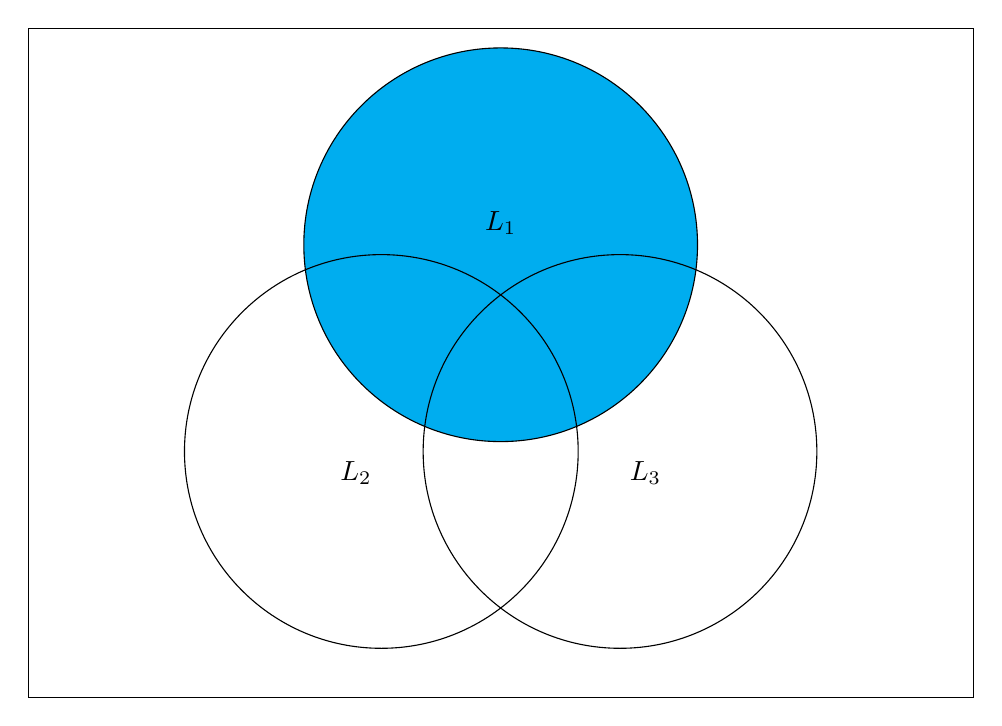
\begin{tikzpicture}
    \draw (-6,-4) rectangle (6,4.5);
      \begin{scope}
    \clip \secondcircle;
      \end{scope}
      \begin{scope}
    \clip \firstcircle;
    \fill[cyan] \firstcircle;
      \end{scope}
      \draw \firstcircle node[text=black,above] {$L_1$};
      \draw \secondcircle node [text=black,below left] {$L_2$};
      \draw \thirdcircle node [text=black,below right] {$L_3$};
    \end{tikzpicture}

    %second venn diagram
    \begin{itemize} [label=\ding{212}]
        \item Next, to satisfy $L_2$, we want to remove all the possible words generated by $L_1 \cap L_2$ from our updated venn diagram from the previous operation, which is reflected by the venn diagram below. 
    \end{itemize}
       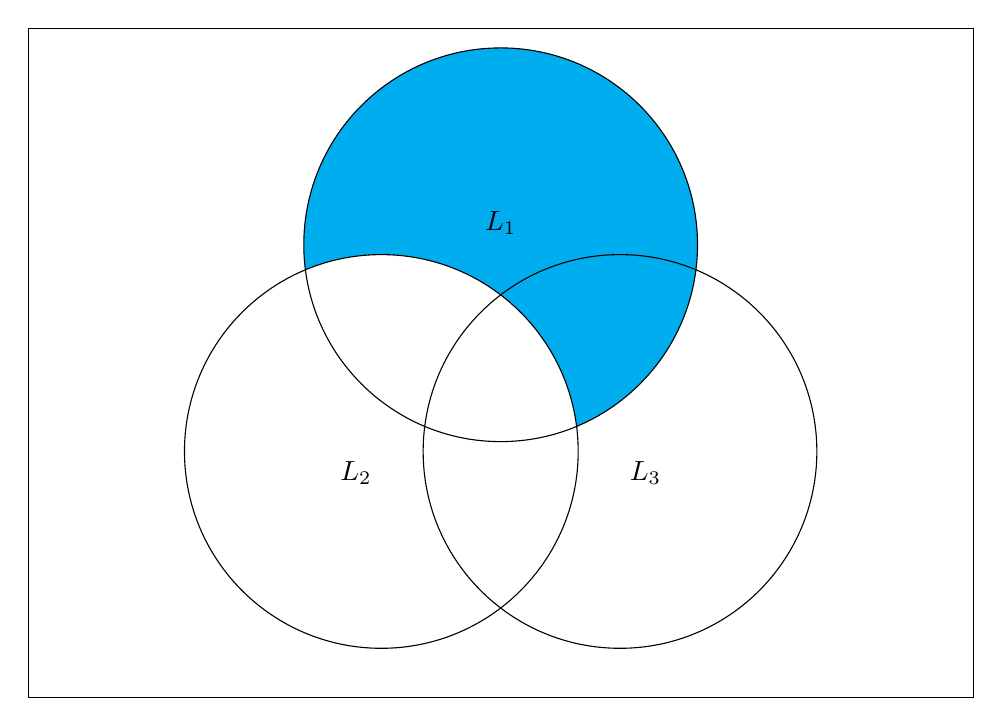
\begin{tikzpicture}
    \draw (-6,-4) rectangle (6,4.5);
      \begin{scope}
    \clip \secondcircle;
      \end{scope}
      \begin{scope}
    \clip \firstcircle;
    \fill[cyan] \firstcircle;
    \fill[white] \secondcircle;
      \end{scope}
      \draw \firstcircle node[text=black,above] {$L_1$};
      \draw \secondcircle node [text=black,below left] {$L_2$};
      \draw \thirdcircle node [text=black,below right] {$L_3$};
    \end{tikzpicture}

    %third venn diagram
    \begin{itemize} [label=\ding{212}]
        \item Finally, to satisfy $L_3$, we want to remove all the possible words generated by $L_1 \cap L_3$ which is reflected by the venn diagram below.
    \end{itemize}
       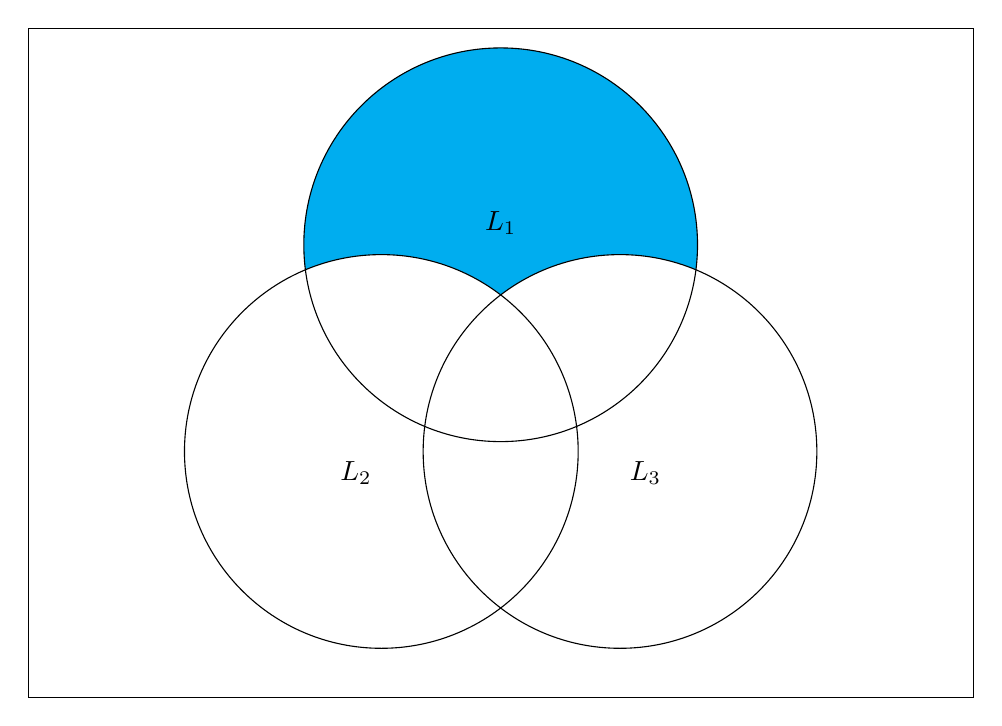
\begin{tikzpicture}
    \draw (-6,-4) rectangle (6,4.5);
      \begin{scope}
    \clip \secondcircle;
      \end{scope}
      \begin{scope}
    \clip \firstcircle;
    \fill[cyan] \firstcircle;
    \fill[white] \secondcircle;
    \fill[white] \thirdcircle;
      \end{scope}
      \draw \firstcircle node[text=black,above] {$L_1$};
      \draw \secondcircle node [text=black,below left] {$L_2$};
      \draw \thirdcircle node [text=black,below right] {$L_3$};
    \end{tikzpicture}
\item In summation, we can describe the language $L_F$ as the language generated by $L_1 - (L_2 \cup L_3)$. And because $L_1$,$L_2$, and $L_3$ are all regular languages closed under set operations union and difference, the language $L_F$ must also be a regular language. 



\begin{proof}[\unskip\nopunct]

\end{proof}

\end{solution}

\newpage

% \vskip 2em 
% \hrule
% \vskip 2em 

% --------------
% Exercise 4
% --------------
\begin{exercise}{4}

Show that the language $L_G$ (described below) is Regular by \textbf{1) constructing a Regular expression} and \textbf{ 2) one finite automaton}.


We will describe language $L_G$ the following way: 

\begin{itemize}
    \item start with all the binary words that have all the zeroes before all the ones;
    \item add all the words that have exactly two ones;
    \item then add all the words that have an even number of zeros;
\end{itemize}

\end{exercise}

% -------------------------------------------
%  Write your answer to Q4 below 1001010
% -------------------------------------------
\begin{solution} \quad
Since the language $L_g$ can be generated by a regular expression and a finite automaton then $L_g$ must be a regular language.\\ 
\\ regular expression: (0*1*)+(0*10*10*)+((00)*1*(00)*1*(00)*)
\begin{center}
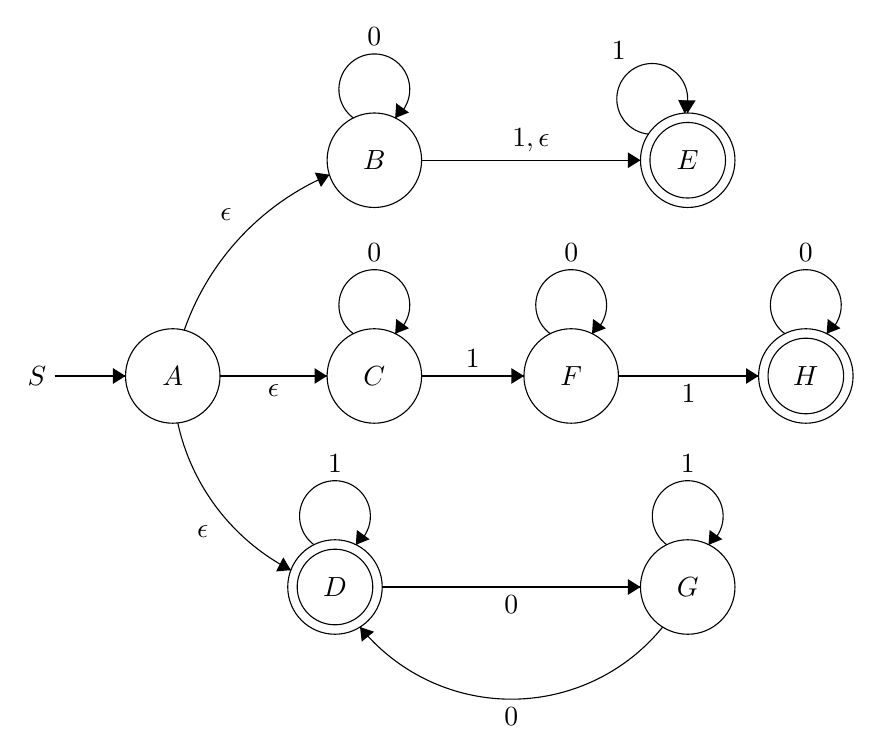
\begin{tikzpicture}[scale=0.2]
\tikzstyle{every node}+=[inner sep=0pt]
\draw [black] (11.1,-28.8) circle (3);
\draw (11.1,-28.8) node {$A$};
\draw [black] (23.9,-15.1) circle (3);
\draw (23.9,-15.1) node {$B$};
\draw [black] (23.9,-28.8) circle (3);
\draw (23.9,-28.8) node {$C$};
\draw [black] (21.4,-42.2) circle (3);
\draw (21.4,-42.2) node {$D$};
\draw [black] (21.4,-42.2) circle (2.4);
\draw [black] (43.8,-15.1) circle (3);
\draw (43.8,-15.1) node {$E$};
\draw [black] (43.8,-15.1) circle (2.4);
\draw [black] (36.4,-28.8) circle (3);
\draw (36.4,-28.8) node {$F$};
\draw [black] (43.8,-42.2) circle (3);
\draw (43.8,-42.2) node {$G$};
\draw [black] (51.3,-28.8) circle (3);
\draw (51.3,-28.8) node {$H$};
\draw [black] (51.3,-28.8) circle (2.4);
\draw [black] (11.829,-25.894) arc (160.78049:113.1098:16.712);
\fill [black] (21.05,-16.02) -- (20.12,-15.88) -- (20.51,-16.8);
\draw (14.87,-18.52) node [left] {$\epsilon$};
\draw [black] (14.1,-28.8) -- (20.9,-28.8);
\fill [black] (20.9,-28.8) -- (20.1,-28.3) -- (20.1,-29.3);
\draw (17.5,-29.3) node [below] {$\epsilon$};
\draw [black] (18.604,-41.128) arc (-117.18976:-167.7144:13.818);
\fill [black] (18.6,-41.13) -- (18.12,-40.32) -- (17.66,-41.21);
\draw (13.39,-38.67) node [left] {$\epsilon$};
\draw [black] (26.9,-15.1) -- (40.8,-15.1);
\fill [black] (40.8,-15.1) -- (40,-14.6) -- (40,-15.6);
\draw (33.85,-14.6) node [above] {$1,\epsilon$};
\draw [black] (26.9,-28.8) -- (33.4,-28.8);
\fill [black] (33.4,-28.8) -- (32.6,-28.3) -- (32.6,-29.3);
\draw (30.15,-28.3) node [above] {$1$};
\draw [black] (39.4,-28.8) -- (48.3,-28.8);
\fill [black] (48.3,-28.8) -- (47.5,-28.3) -- (47.5,-29.3);
\draw (43.85,-29.3) node [below] {$1$};
\draw [black] (22.577,-12.42) arc (234:-54:2.25);
\draw (23.9,-7.85) node [above] {$0$};
\fill [black] (25.22,-12.42) -- (26.1,-12.07) -- (25.29,-11.48);
\draw [black] (22.577,-26.12) arc (234:-54:2.25);
\draw (23.9,-21.55) node [above] {$0$};
\fill [black] (25.22,-26.12) -- (26.1,-25.77) -- (25.29,-25.18);
\draw [black] (35.077,-26.12) arc (234:-54:2.25);
\draw (36.4,-21.55) node [above] {$0$};
\fill [black] (37.72,-26.12) -- (38.6,-25.77) -- (37.79,-25.18);
\draw [black] (49.977,-26.12) arc (234:-54:2.25);
\draw (51.3,-21.55) node [above] {$0$};
\fill [black] (52.62,-26.12) -- (53.5,-25.77) -- (52.69,-25.18);
\draw [black] (20.077,-39.52) arc (234:-54:2.25);
\draw (21.4,-34.95) node [above] {$1$};
\fill [black] (22.72,-39.52) -- (23.6,-39.17) -- (22.79,-38.58);
\draw [black] (42.477,-39.52) arc (234:-54:2.25);
\draw (43.8,-34.95) node [above] {$1$};
\fill [black] (45.12,-39.52) -- (46,-39.17) -- (45.19,-38.58);
\draw [black] (3.6,-28.8) -- (8.1,-28.8);
\draw (3.1,-28.8) node [left] {$S$};
\fill [black] (8.1,-28.8) -- (7.3,-28.3) -- (7.3,-29.3);
\draw [black] (43.8,-12) -- (43.8,-12.1);
\fill [black] (43.8,-12.1) -- (44.3,-11.3) -- (43.3,-11.3);
\draw [black] (41.313,-13.444) arc (264.06858:-23.93142:2.25);
\draw (39.42,-8.76) node [above] {$1$};
\fill [black] (43.6,-12.12) -- (44.18,-11.37) -- (43.19,-11.27);
\draw [black] (42.212,-44.737) arc (-38.98959:-141.01041:12.367);
\fill [black] (22.99,-44.74) -- (23.1,-45.67) -- (23.88,-45.04);
\draw (32.6,-49.82) node [below] {$0$};
\draw [black] (24.4,-42.2) -- (40.8,-42.2);
\fill [black] (40.8,-42.2) -- (40,-41.7) -- (40,-42.7);
\draw (32.6,-42.7) node [below] {$0$};
\end{tikzpicture}
\end{center}
\paragraph{
We tested the following edge cases for the final constraint:
}
\begin{enumerate}
    \item 0000
    \item 1111
    \item 100100
    \item 000
\end{enumerate}
\end{solution}

% -----------------
% References
% -----------------
\vfill
\begin{thebibliography}{9}
 \bibitem{sipser} 
Sipser, Michael. 
\textit{Introduction to the Theory of Computation.}
Course Technology, 2005. ISBN: 9780534950972

\bibitem{critchlow2011foundation}
Critchlow, Carol and Eck, David
\textit{Foundation of computation.},
Critchlow Carol, 2011
\end{thebibliography}


% --------------------------------------------------------------
%     You don't have to mess with anything below this line.
% --------------------------------------------------------------
 
\end{document}